\documentclass[]{report}   % list options between brackets        
\usepackage{graphicx, listings, color}      % list packages between braces
\graphicspath{ {Images/} }

% type user-defined commands here

\definecolor{codegreen}{rgb}{0,0.6,0}
\definecolor{codegray}{rgb}{0.5,0.5,0.5}
\definecolor{codepurple}{rgb}{0.58,0,0.82}
\definecolor{backcolour}{rgb}{0.95,0.95,0.92}
 
\lstdefinestyle{mystyle}{
    backgroundcolor=\color{backcolour},   
    commentstyle=\color{codegreen},
    keywordstyle=\color{magenta},
    numberstyle=\tiny\color{codegray},
    stringstyle=\color{codepurple},
    basicstyle=\footnotesize,
    breakatwhitespace=false,         
    breaklines=true,                 
    captionpos=b,                    
    keepspaces=true,                 
    numbers=left,                    
    numbersep=5pt,                  
    showspaces=false,                
    showstringspaces=false,
    showtabs=false,                  
    tabsize=2
}
 
\lstset{style=mystyle}

\begin{document}

\title{CAB420 Assignment 1}   % type title between braces
\author{Jarrod Williams (n9722068) and Madeline Miller (n9342401)}         % type author(s) between braces
\maketitle

\chapter{Theory}

Given the following equation,

$$L(w)=-\sum_{i=1}^{N}log(\frac{1}{1+e^{y_i(w^Tx_i+b)}})+\lambda||w||_2^2$$

\section{Finding the Partial Derivative}
Finding the partial derivative $$\frac{\partial L}{\partial w_j}$$

$$\frac{\partial L}{\partial w_j}(-\sum_{i=1}^{N}log(\frac{1}{1+e^{y_i(w^Tx_i+b)}})+\lambda||w||_2^2)$$

As the regulator at the end of the function is a squared L2 norm, it can be derived trivially.

$$\frac{\partial L}{\partial w_j}(-\sum_{i=1}^{N}log(\frac{1}{1+e^{y_i(w^Tx_i+b)}}))+2\lambda w_j$$

Simplify,

$$\frac{\partial L}{\partial w_j}(\sum_{i=1}^{N}log(1+e^{y_i(w^Tx_i+b)}))+2\lambda w_j$$

Using the chain rule,

$$\sum_{i=1}^{N}\frac{\frac{\partial L}{\partial w_j}(1+e^{y_i(w^Tx_i+b)})}{1+e^{y_i(w_jx_{i,j}+b)}}+2\lambda w_j$$

$$\sum_{i=1}^{N}\frac{\frac{\partial L}{\partial w_j}(1)+\frac{\partial L}{\partial w_j}(e^{y_i(w^Tx_i+b)})}{1+e^{y_i(w_jx_{i,j}+b)}}+2\lambda w_j$$

$$\sum_{i=1}^{N}\frac{\frac{\partial L}{\partial w_j}(e^{y_i(w^Tx_i+b)})}{1+e^{y_i(w_jx_{i,j}+b)}}+2\lambda w_j$$

Using the chain rule again,

$$\sum_{i=1}^{N}\frac{y_ix_ie^{y_i(w^Tx_i+b)}}{1+e^{y_i(w_jx_{i,j}+b)}}+2\lambda w_j$$

\section{Finding the Second Partial Derivative}
Finding the second partial derivative $$\frac{\partial^2 L}{\partial w_j\partial w_k}$$

$$\frac{\partial^2 L}{\partial w_j\partial w_k}=\frac{\partial}{\partial w_k}(\sum_{i=1}^{N}\frac{y_ix_ie^{y_i(w^Tx_i+b)}}{1+e^{y_i(w_jx_{i,j}+b)}}+2\lambda w_j)$$

$$\frac{\partial}{\partial w_k}(\sum_{i=1}^{N}\frac{y_ix_ie^{y_i(w^Tx_i+b)}}{1+e^{y_i(w_jx_{i,j}+b)}})$$

$$\sum_{i=1}^{N}\frac{y_ix_i(\frac{\partial}{\partial w_k}e^{y_i(w^Tx_i+b)})}{1+e^{y_i(w_jx_{i,j}+b)}}$$

Using the chain rule,

$$\sum_{i=1}^{N}\frac{e^{y_i(w_kx_i+b)}y_i^2x_i(\frac{\partial}{\partial w_k}(w^Tx_i+b))}{1+e^{y_i(w_jx_{i,j}+b)}}$$

$$\sum_{i=1}^{N}\frac{e^{y_i(w^Tx_i+b)}y_i^2x_iw_kx_i+b}{1+e^{y_i(w_jx_{i,j}+b)}}$$

$$\sum_{i=1}^{N}\frac{e^{y_i(w^Tx_i+b)}y_i^2x_i^2w_k+b}{1+e^{y_i(w_jx_{i,j}+b)}}$$

\section{Proving it's a convex function}

A function can be defined as convex if the Hessian matrix is positive semi-definite. This is defined as,

$$a^THa\equiv\sum_{j,k}a_ja_kH_{j,k}\geq0$$

Where,

$$H_{j,k}=\frac{\partial^2L}{\partial w_j\partial w_k}$$

Using proof by contradiction, 




\chapter{Practice}


\section{Features, Classes, and Linear Regression}
%%%%%%%%%%%%%%%%%%%%
(a) Plot the training data in a scatter plot.
\begin{center}
	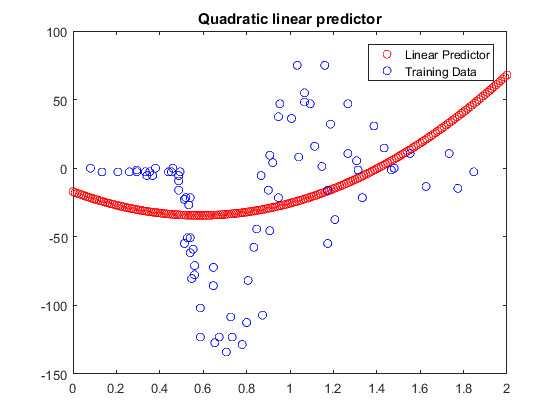
\includegraphics[width=35em]{2_1_Figure_1.png}
	{Figure 1: Training data in a scatter plot.}
\end{center} 
~\\
(b) Create a linear predictor (assuming quadratic features). Plot it on the same plot as the training data.
\begin{center}
	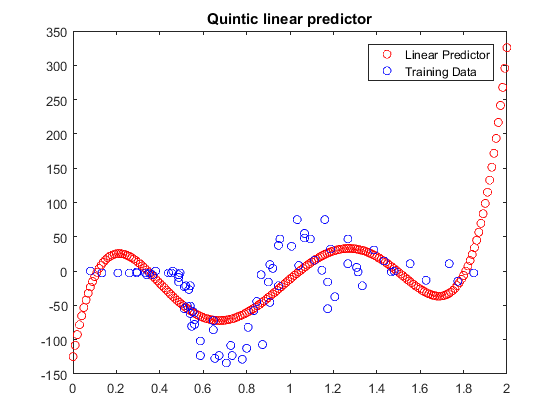
\includegraphics[width=35em]{2_1_Figure_2.png}
	{Figure 2: Quadratic linear predictor with training data scatter plot.}
\end{center}.
~\\ 
(c) Create another plot with the data and a fifth-degree polynomial.
\begin{center}
	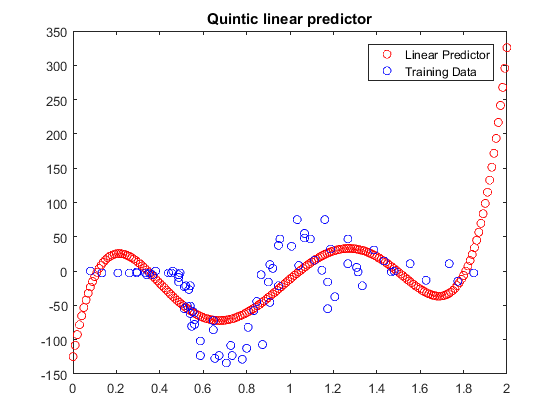
\includegraphics[width=35em]{2_1_Figure_3.png}
	{Figure 3: Quintic linear predictor with training data scatter plot.}
\end{center}
~\\
(d) Calculate the mean squared error associated with each of your learned models on the training
data.
\begin{lstlisting}[caption=Matlab output for MSE calculations on training data.]
The MSE for the quadratic linear predictor on training data was: 2178.55
The MSE for the quintic linear predictor on training data was: 1254.61
\end{lstlisting}
~\\
(e) Calculate the MSE for each model on the test data (in mcycleTest.txt).
\begin{lstlisting}[caption=Matlab output for MSE calculations on test data.]
The MSE for the quadratic linear predictor on test data was: 1573.27
The MSE for the quintic linear predictor on test data was: 999.65
\end{lstlisting}





\section{kNN Regression}
\section{Hold-out and Cross-validation}
\section{Nearest Neighbor Classifiers}
%%%%%%%%%%%%%%%%%%%%
(a) Plot the data by their feature values, using the class value to select the color.
\begin{center}
	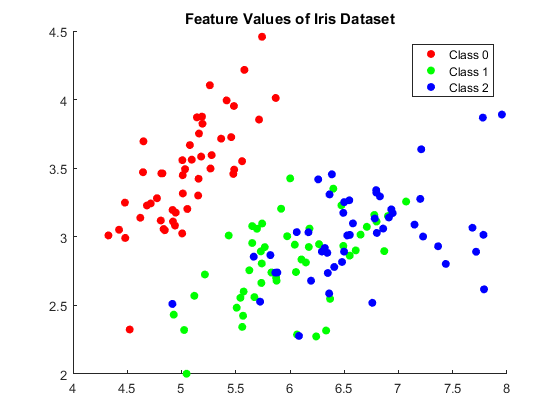
\includegraphics[width=35em]{2_4_Figure_1.png}
	{Figure X: Data plotted by feature value with class value determining colour.}
\end{center} 
~\\
(b) Use the provided $knnClassify$ class to learn a 1-nearest-neighbour predictor. Use the function $class2DPlot(learner,X,Y)$ to plot the decision regions and training data together.
\begin{lstlisting}[language=Matlab, caption=Teaching the 1-nearest-neighbour predictor.]
learner = knnClassify(1, X, Y);
class2DPlot(learner,X,Y);
title('1-nearest-neighbour predictor');
\end{lstlisting}
\begin{center}
	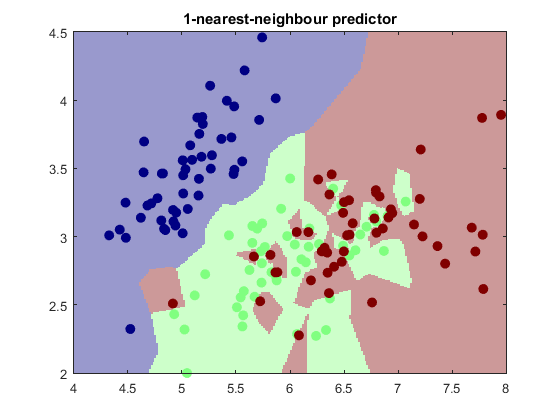
\includegraphics[width=35em]{2_4_Figure_2.png}
	{Figure 3: Plot of decision regions and training data. Generated with $class2DPlot()$.}
\end{center} 
~\\
(c) Do the same thing for several values of k (say, [1, 3, 10, 30]) and comment on their appearance.
\begin{center}
	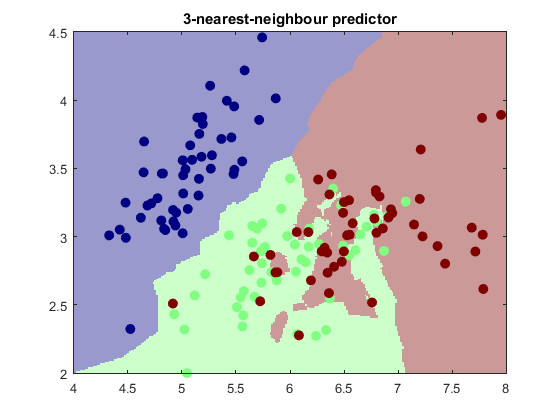
\includegraphics[width=35em]{2_4_Figure_3.png}
\end{center} 
\begin{center}
	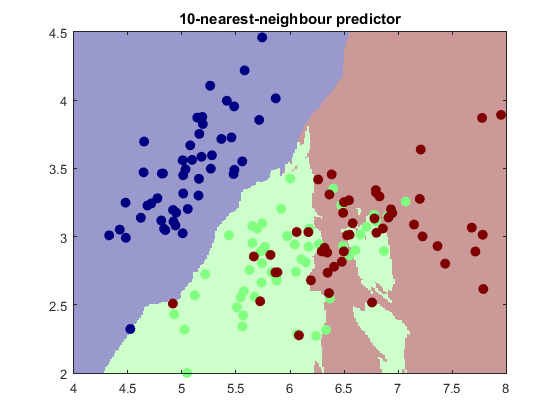
\includegraphics[width=35em]{2_4_Figure_4.png}
\end{center} 
\begin{center}
	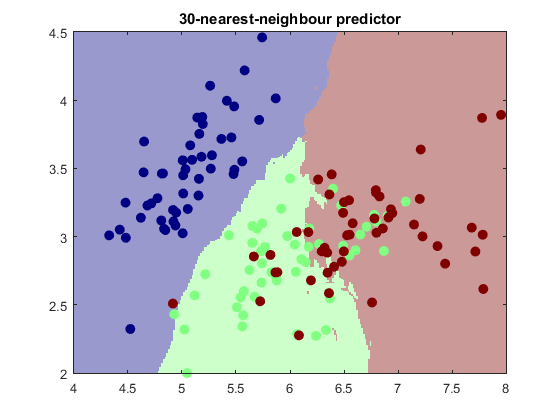
\includegraphics[width=35em]{2_4_Figure_5.png}
\end{center} 
{As the value of $k$ increases, so does the definition of the decision regions. At small values of $k$, under-fitting occurs. At large values of $k$, over-fitting occurs.}
\\~\\
{(d) Now split the data into an 80/20 training/validation split. For k = [1, 2, 5, 10, 50, 100, 200], learn a model on the 80$\%$ and calculate its performance ($\#$ of data classified incorrectly) on the validation data.}
\begin{center}
	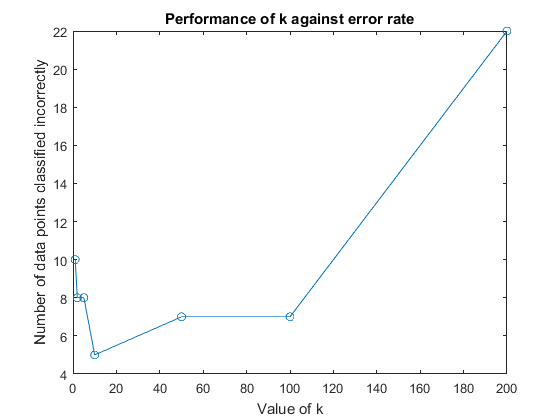
\includegraphics[width=35em]{2_4_Figure_6.png}
\end{center} 
{What value of k appears to generalize best given your training data? Comment on the performance at the two endpoints, in terms of over- or under-fitting.} \\~\\
{Where small values of $k$ underfit (1,3,5) and large values overfit (100,200), where $k = 10$ appears to generalise best.}



\section{Perceptrons and Logistic Regression}
{(a) Show the two classes in a scatter plot and verify that one is linearly separable while the other is not.}
\begin{center}
%	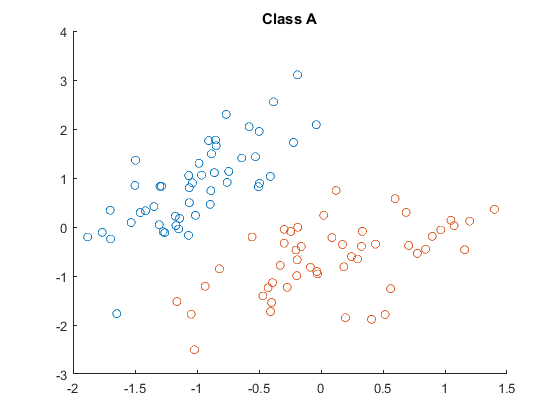
\includegraphics[width=35em]{2_5_Figure_1.png}
	{Figure X: Class A. Data {\bf is} linearly separable.}
\end{center} 
\begin{center}
%	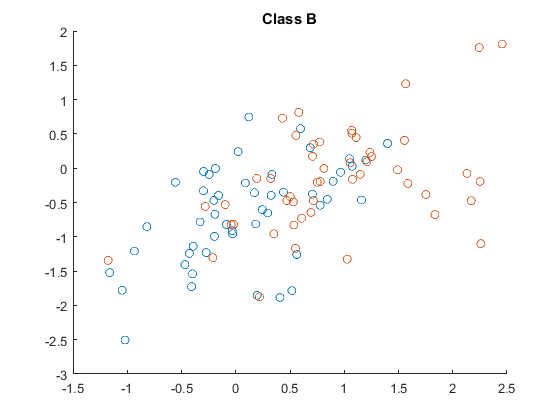
\includegraphics[width=35em]{2_5_Figure_2.png}
	{Figure X: Class B. Data {\bf is not} linearly separable.}
\end{center} 
{(b) Write the function @logisticClassify2/plot2DLinear.m so that it plots the two
classes of data in different colors, along with the decision boundary. Include the listing of your code in your report.}

\begin{lstlisting}[language=Matlab, caption=plot2DLinear() Implementation]
function plot2DLinear(obj, X, Y)
% plot2DLinear(obj, X,Y)
%   plot a linear classifier (data and decision boundary) when features X are 2-dim
%   wts are 1x3,  wts(1)+wts(2)*X(1)+wts(3)*X(2)
%
[n,d] = size(X);
if (d~=2) error('Sorry -- plot2DLogistic only works on 2D data...'); end;

%%% TODO: Fill in the rest of this function...
figure('Name','Linear Plot');
hold on;

% Plot class data.
classes = unique(Y);

classAIndicies = find(Y==classes(1));
xPointsClassA = X(classAIndicies, 1:end);
scatter(xPointsClassA(:, 1), xPointsClassA(:, 2));

classBIndicies = find(Y==classes(2));
xPointsClassB = X(classBIndicies, 1:end);
scatter(xPointsClassB(:, 1), xPointsClassB(:, 2));


% Plot decision boundary.
wts = getWeights(obj);
f = @(x1, x2) wts(1) + wts(2)*x1 + wts(3)*x2 ;
ezplot(f,[-3.5,3.5])

legend('Class 0','Class 1', 'Decision Bondary');
hold off;
\end{lstlisting}
{To demo your function plot the decision boundary corresponding to the classifier: $sign( .5 + 1x_{1} − .25x_{2} )$ along with the A data, and again with the B data.}
\begin{lstlisting}[language=Matlab, caption=Demoing plot2DLinear()]
%% (B) Write the function @logisticClassify2/plot2DLinear.m such that it 
%      can Plot the two classes of data in different colors, along with the 
%      decision boundary (a line). To demo your function plot the decision 
%       boundary corresponding to the classifier sign( .5 + 1x1 − .25x2 )
%       along with the A data, and again with the B data.

learner=logisticClassify2(); % create "blank" learner
learner=setClasses(learner, unique(YA)); % define class labels using YA or YB
wts = [0.5 1 -0.25]; % TODO: fill in values
learner=setWeights(learner, wts); % set the learner's parameters
plot2DLinear(learner, XA, YA);
title('Class A with Decision Boundary');
plot2DLinear(learner, XB, YB);
title('Class B with Decision Boundary');
\end{lstlisting}
\begin{center}
%	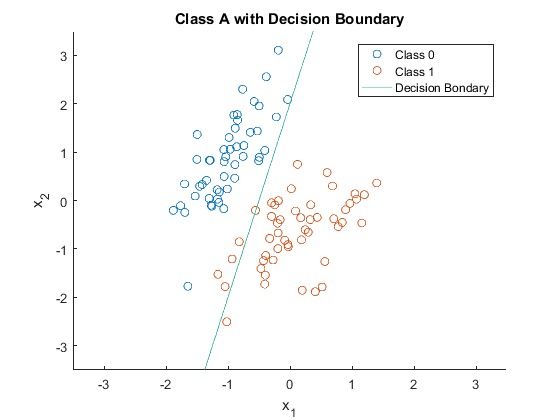
\includegraphics[width=35em]{2_5_Figure_3.png}
	{Figure X: Class A with decision boundary plotted.}
\end{center} 
\begin{center}
%	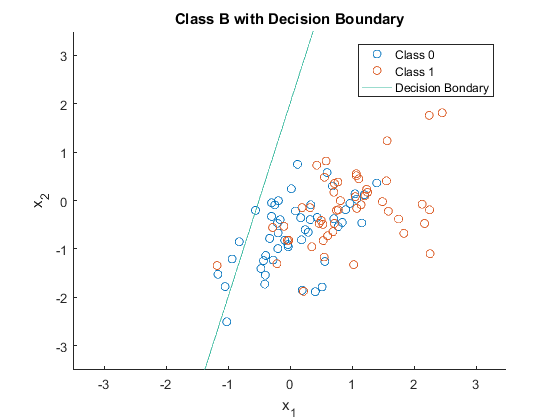
\includegraphics[width=35em]{2_5_Figure_4.png}
	{Figure X: Class B with decision boundary plotted.}
\end{center} 
{(c) Complete the predict.m function to make predictions for your linear classifier.}
\begin{lstlisting}[language=Matlab, caption=predict() Implementation]
function Yte = predict(obj,Xte)
% Yhat = predict(obj, X)  : make predictions on test data X

% (1) make predictions based on the sign of wts(1) + wts(2)*x(:,1) + ...
% (2) convert predictions to saved classes: Yte = obj.classes( [1 or 2] );
wts = getWeights(obj);
yhat = zeros(size(Xte,1),1);
f = @(x1, x2) wts(1) + wts(2)*x1 + wts(3)*x2;

for i=1:size(Xte,1)
    x = sign(f(Xte(i,1),Xte(i,2)));
    yhat(i) = obj.classes(ceil((x+3)/2));
end;

Yte = yhat;
\end{lstlisting}
{Again, verify that your function works by computing \& reporting the error rate of the classifier in the previous part on both data sets A and B. (The error rate on data set A should be ≈ 0.0505.)}
\begin{lstlisting}[language=Matlab, caption=Verifying predict() works]
yte = predict(learner,XA);
classError = errorTrain(YA,yte); % = 0.0505
disp(strcat({'The error for class A is:'},{' '},{num2str(classError,' %.4f')}));

yte = predict(learner,XB);
classError = errorTrain(YB,yte); % = 0.5455
disp(strcat({'The error for class B is:'},{' '},{num2str(classError,' %.4f')}));
\end{lstlisting}
\begin{center}
	{Output from Listing 2.4 is as follows: \\ 'The error for class A is: 0.0505' \\ 'The error for class B is: 0.5455'.}
\end{center} 
{(d) The derivative of the gradient can be found by computing xxx over the surrogate loss for point ji. The derivative then is as follows:
}



(e) Complete your train.m function to perform stochastic gradient descent on the logistic loss function. This will require that you fill in:

(1) computing the surrogate loss function at each iteration ($J = 1/m\sum J_{j}$)



(2) computing the prediction and gradient associated with each data point x
(i)
, y(i)
;
(3) a gradient step on the parameters θ;
(4) a stopping criterion (usually either stopIter iterations or that J has not changed by more
than stopTol since the last iteration through all the data).

\end{document}
